\documentclass[aspectratio=169]{beamer}

% ============================================================================
% PACKAGES
% ============================================================================
\usepackage[utf8]{inputenc}
\usepackage{amsmath}
\usepackage{amssymb}
\usepackage{booktabs}
\usepackage{array}
\usepackage{graphicx}
\usepackage{tikz}
\usetikzlibrary{arrows.meta, positioning}
\usepackage{xcolor}

% ============================================================================
% THEME: custom formal navy/white theme (matches department review template)
% ============================================================================
\usetheme{default}
\setbeamertemplate{navigation symbols}{}
\setbeamertemplate{itemize items}[circle]

\definecolor{iiitblue}{RGB}{10,55,120}
\definecolor{iiitgray}{RGB}{90,90,90}

\setbeamercolor{frametitle}{bg=iiitblue,fg=white}
\setbeamercolor{title}{fg=iiitblue}
\setbeamercolor{structure}{fg=iiitblue}
\setbeamercolor{normal text}{fg=black}
\setbeamerfont{frametitle}{series=\bfseries,size=\large}

% Path to the extracted institute logo (same folder as this .tex file)
\newcommand{\iiitlogo}{logo_extract-000.png}

% --- Custom frame title: blue bar spanning the slide, logo on the right ---
\setbeamertemplate{frametitle}{
  \nointerlineskip
  \begin{beamercolorbox}[wd=\paperwidth,ht=1.15cm,dp=0.35cm,leftskip=0.4cm,rightskip=0.3cm]{frametitle}
    \begin{minipage}[c]{0.82\textwidth}
      \raggedright\insertframetitle
    \end{minipage}%
    \hfill
    \begin{minipage}[c]{0.14\textwidth}
      \raggedleft\includegraphics[height=0.85cm]{\iiitlogo}
    \end{minipage}
  \end{beamercolorbox}
}

% --- Custom footline: author | institute | page number ---
\setbeamertemplate{footline}{
  \leavevmode
  \hbox{%
    \begin{beamercolorbox}[wd=.33\paperwidth,ht=2.6ex,dp=1.2ex,left,leftskip=0.4cm]{footline}
      {\color{iiitblue}\tiny Joel James P \& Syeda Majida Bee}
    \end{beamercolorbox}%
    \begin{beamercolorbox}[wd=.34\paperwidth,ht=2.6ex,dp=1.2ex,center]{footline}
      {\color{iiitgray}\tiny Indian Institute of Information Technology Kottayam}
    \end{beamercolorbox}%
    \begin{beamercolorbox}[wd=.33\paperwidth,ht=2.6ex,dp=1.2ex,right,rightskip=0.4cm]{footline}
      {\color{iiitblue}\tiny \insertframenumber{} / \inserttotalframenumber}
    \end{beamercolorbox}%
  }
  \vskip 0.6ex
}

\setbeamertemplate{blocks}[rounded][shadow=false]

% ============================================================================
% TITLE INFO
% ============================================================================
\title{Intelligent Mode Selection for Dual-Functional Radar-Communication in Autonomous Vehicles}
\author{Joel James P \& Syeda Majida Bee}
\institute{Department of Electronics and Communication Engineering\\Indian Institute of Information Technology Kottayam}
\date{}

\begin{document}

% ============================================================================
% TITLE SLIDE (custom, matches department review-1 format)
% ============================================================================
\begin{frame}[plain]
  \vspace{0.1cm}
  \begin{center}
    \includegraphics[height=1.3cm]{\iiitlogo}\\[0.35cm]
    {\Large\bfseries\color{iiitblue} Intelligent Mode Selection for Dual-Functional\\ Radar-Communication in Autonomous Vehicles}\\[0.5cm]
    \begin{tabular}{>{\centering\arraybackslash}p{4.3cm} c >{\centering\arraybackslash}p{4.3cm}}
      \bfseries Joel James P & \normalsize by & \bfseries Syeda Majida Bee \\
      \small 2023BEC0010 & & \small 2023BEC0040 \\
    \end{tabular}\\[0.35cm]
    {\small Department of Electronics and Communication Engineering}\\
    {\small Indian Institute of Information Technology Kottayam}\\[0.3cm]
    \begin{tabular}{>{\centering\arraybackslash}p{4.3cm} >{\centering\arraybackslash}p{6.3cm}}
      \small Internal Guide, & \small External Guide, \\
      \bfseries Dr. Ananth A & \bfseries Dr. Pradyumna Kumar Bishoyi \\
    \end{tabular}\\[0.4cm]
    {\small BTP Review 1}
  \end{center}
\end{frame}

% ============================================================================
% OUTLINE
% ============================================================================
\begin{frame}{Presentation Outline}
  \centering
  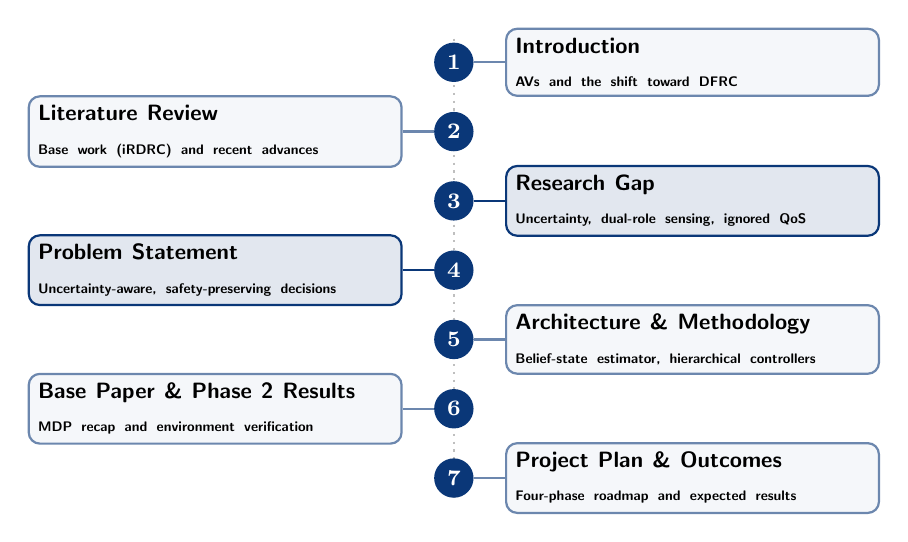
\begin{tikzpicture}[
    font=\sffamily,
    circ/.style={circle, fill=iiitblue, text=white, font=\bfseries\footnotesize, minimum size=0.5cm, inner sep=0pt},
    plainbox/.style={draw=iiitblue!60, thick, rounded corners, fill=iiitblue!4,
      minimum height=0.66cm, font=\sffamily},
    hlbox/.style={draw=iiitblue, thick, rounded corners, fill=iiitblue!12,
      minimum height=0.66cm, font=\sffamily},
  ]

  \def\ny{2.5} \def\dy{0.88}

  % --- central dotted line ---
  \draw[gray!50, dotted, thick] (0,\ny+0.3) -- (0,\ny-6*\dy-0.3);

  % --- circles ---
  \foreach \i/\y in {1/\ny, 2/{\ny-\dy}, 3/{\ny-2*\dy}, 4/{\ny-3*\dy}, 5/{\ny-4*\dy}, 6/{\ny-5*\dy}, 7/{\ny-6*\dy}} {
    \node[circ] (c\i) at (0,\y) {\i};
  }

  % --- right-side boxes: 1, 3, 5, 7 ---
  \node[plainbox, anchor=west, text width=4.5cm, align=left] (b1) at (0.65,\ny)
    {\footnotesize\bfseries Introduction \\ {\tiny\itshape AVs and the shift toward DFRC}};
  \node[hlbox, anchor=west, text width=4.5cm, align=left] (b3) at (0.65,{\ny-2*\dy})
    {\footnotesize\bfseries Research Gap \\ {\tiny\itshape Uncertainty, dual-role sensing, ignored QoS}};
  \node[plainbox, anchor=west, text width=4.5cm, align=left] (b5) at (0.65,{\ny-4*\dy})
    {\footnotesize\bfseries Architecture \& Methodology \\ {\tiny\itshape Belief-state estimator, hierarchical controllers}};
  \node[plainbox, anchor=west, text width=4.5cm, align=left] (b7) at (0.65,{\ny-6*\dy})
    {\footnotesize\bfseries Project Plan \& Outcomes \\ {\tiny\itshape Four-phase roadmap and expected results}};

  % --- left-side boxes: 2, 4, 6 ---
  \node[plainbox, anchor=east, text width=4.5cm, align=left] (b2) at (-0.65,{\ny-\dy})
    {\footnotesize\bfseries Literature Review \\ {\tiny\itshape Base work (iRDRC) and recent advances}};
  \node[hlbox, anchor=east, text width=4.5cm, align=left] (b4) at (-0.65,{\ny-3*\dy})
    {\footnotesize\bfseries Problem Statement \\ {\tiny\itshape Uncertainty-aware, safety-preserving decisions}};
  \node[plainbox, anchor=east, text width=4.5cm, align=left] (b6) at (-0.65,{\ny-5*\dy})
    {\footnotesize\bfseries Base Paper \& Phase 2 Results \\ {\tiny\itshape MDP recap and environment verification}};

  % --- connectors ---
  \draw[iiitblue!60, thick] (c1) -- (b1.west);
  \draw[iiitblue!60, thick] (c2) -- (b2.east);
  \draw[iiitblue, thick] (c3) -- (b3.west);
  \draw[iiitblue, thick] (c4) -- (b4.east);
  \draw[iiitblue!60, thick] (c5) -- (b5.west);
  \draw[iiitblue!60, thick] (c6) -- (b6.east);
  \draw[iiitblue!60, thick] (c7) -- (b7.west);

  \end{tikzpicture}
\end{frame}

% ============================================================================
% ============================  INTRODUCTION  ===============================
% ============================================================================

% --- Intro Slide 1: AVs and their sensing/communication needs ---
\begin{frame}{Introduction: Why Autonomous Vehicles Need Both Radar and Communication}
  \textbf{Autonomous Vehicles (AVs) rely on two distinct but hardware-similar subsystems:}
  \begin{itemize}
    \item \textbf{Radar (Sensing):} Detects obstacles, pedestrians, and hazards in real time. Critical for collision avoidance, especially in poor visibility (rain, fog, night).
    \item \textbf{Communication (V2X/V2I):} Transmits sensor data, traffic status, and telemetry to edge/cloud infrastructure or nearby vehicles for cooperative driving, route planning, and remote monitoring.
  \end{itemize}

  \vspace{0.3cm}
  \textbf{The core tension:}
  \begin{itemize}
    \item Both functions increasingly share the same RF front-end, spectrum band, and hardware (mmWave radios also make good radars).
    \item An AV cannot always do both at once with limited hardware --- every time slot spent communicating is a time slot \emph{not} spent sensing, and vice versa.
    \item This shared-resource conflict motivates \textbf{Dual-Functional Radar-Communication (DFRC)} systems.
  \end{itemize}
\end{frame}

% --- Intro Slide 2: Evolution of radar-communication integration ---
\begin{frame}{Evolution: From Separate Systems to Joint Radar-Communication}
  \small
  \begin{enumerate}
    \item \textbf{Separate Systems (Traditional):} Dedicated radar hardware + dedicated communication radio, operating on different spectrum. Simple, but costly, bulky, and spectrum-inefficient as vehicular spectrum demand grows.
    \item \textbf{Spectrum Congestion Pressure:} Growing V2X traffic and radar density (multiple AVs, mmWave bands) pushed research toward \textbf{sharing} hardware/spectrum instead of duplicating it.
    \item \textbf{Joint Radar-Communication (JRC) / DFRC:} A single hardware platform performs both functions, saving cost, size, and power --- the foundation of modern automotive DFRC research.
    \item \textbf{Fixed / Scheduled Sharing (Early DFRC):} Static time-cycle division or preamble-based reservation (e.g., 802.11ad-style schemes) --- radar and comm get a pre-agreed fixed share of time, regardless of actual need.
    \item \textbf{Adaptive, Learned Sharing (Current Direction):} Since road conditions, traffic, and weather change dynamically, a \textbf{learned, adaptive policy} decides mode selection in real time --- this is the direction our base paper (iRDRC) takes.
  \end{enumerate}
\end{frame}

% --- Intro Slide 3: Why fixed scheduling falls short ---
\begin{frame}{Why Fixed Scheduling Falls Short}
  \textbf{Static/scheduled resource-sharing assumes a predictable world. Reality is not predictable:}
  \begin{itemize}
    \item \textbf{Weather and road conditions} change continuously --- a fixed radar/comm ratio that works on a clear highway is unsafe in fog or on a wet, winding road.
    \item \textbf{Traffic and moving-object density} varies --- more radar time is needed near pedestrians/intersections; more comm time is fine on an empty highway.
    \item \textbf{Channel quality} fluctuates --- a fixed schedule wastes comm slots on a bad channel and under-uses a good one.
    \item Fixed schemes cannot trade off \textbf{throughput vs. safety} on the fly --- they are tuned once, offline, for an average case.
  \end{itemize}

  \vspace{0.3cm}
  \textbf{Consequence:} The system either wastes capacity (over-cautious radar use) or risks missed hazards (over-aggressive comm use). This motivates replacing fixed rules with a \textbf{learned, state-aware decision policy}.
\end{frame}

% --- Intro Slide 4: Bridge to DFRC + intelligent mode selection ---
\begin{frame}{Toward Intelligent, Adaptive DFRC}
  \textbf{The shift in this line of research:}
  \begin{itemize}
    \item Treat mode selection (radar vs.\ communication) as a \textbf{sequential decision-making problem}, not a fixed schedule.
    \item At every time step, the AV observes its situation --- queue backlog, channel quality, road/weather/speed/traffic conditions --- and \textbf{decides} which mode to use.
    \item This naturally maps to a \textbf{Markov Decision Process (MDP)}, solved using reinforcement learning (e.g., Deep Q-Networks).
  \end{itemize}

  \vspace{0.3cm}
  \textbf{This is exactly the approach of our base paper:}
  \begin{center}
    \textit{iRDRC --- An Intelligent Real-Time Dual-Functional Radar-Communication System for Automotive Vehicles} (Hieu et al., IEEE Wireless Communications Letters, 2020)
  \end{center}
  \small Next: a closer look at this base work, followed by recent papers that build on the same idea.
\end{frame}

% ============================================================================
% ==========================  LITERATURE REVIEW  ============================
% ============================================================================

% --- Lit Review Slide 1: Base work ---
\begin{frame}{Literature Review: Base Work --- iRDRC (Hieu et al., 2020)}
  \small
  \textbf{iRDRC} models the AV's radar/communication choice as an \textbf{MDP} $\langle S, A, R, P, \gamma \rangle$:
  \begin{itemize}
    \item \textbf{State:} $(d, c, r, w, v, m)$ --- data queue length, channel quality, and four binary environmental risk factors (road, weather, speed, moving objects); 352 discrete states.
    \item \textbf{Action:} Binary choice each time step --- communicate ($a=0$) or scan with radar ($a=1$).
    \item \textbf{Reward:} Safety-first design --- small positive reward for successful communication, a large penalty ($-50$) for missing a hazard while communicating, and a risk-scaled reward for successful radar detection.
    \item \textbf{Solver:} Deep Q-Network (DQN) learns the optimal policy $\pi^*(s)$ from experience, without needing a hand-crafted schedule.
  \end{itemize}
  \vspace{0.15cm}
  \textbf{Significance:} First to frame automotive DFRC mode-selection as a \emph{learned} policy rather than a fixed/static allocation --- the direct foundation for this project.
\end{frame}

% --- Lit Review Slide 2: Recent works building on this idea ---
\begin{frame}{Literature Review: Recent Advances Building on This Idea}
  \tiny
  \begin{tabular}{p{2.6cm}p{2.6cm}p{6.3cm}}
    \toprule
    \textbf{Reference} & \textbf{Approach} & \textbf{Modification / Extension over iRDRC-style single-AV DQN} \\
    \midrule
    Lee et al. (2022), \textit{IEEE TVT} & Graph Neural Network (GNN) for JRC & Moves from a single-AV binary decision to a \textbf{multi-vehicle cooperative} setting; needs \textbf{minimal prior system-model knowledge}; introduces a \textbf{data-usefulness metric} to decide what/whom to transmit to, with a tunable radar-comm performance balance. \\
    \addlinespace
    Li et al. (2024), \textit{IEEE (THz-JSAC)} & Dynamic GNN for THz sensing + comm & Extends to \textbf{Terahertz-band} joint sensing-communication across a \textbf{vehicular network} (not one AV); each vehicle can offer sensing-only, comm-only, or \textbf{both}; a topology-adaptive dynamic GNN outperforms static GNN/optimization baselines by 17--28\%. \\
    \addlinespace
    IEEE TVT (2024) & Hybrid DDPG + DQN for ISAC resource allocation & Replaces the single binary DQN action with a \textbf{hybrid continuous + discrete} action space: DDPG allocates channel/power (continuous), DQN allocates bandwidth (discrete), jointly across \textbf{many vehicles} under spectrum scarcity. \\
    \bottomrule
  \end{tabular}

  \vspace{0.2cm}
  \small\textbf{Common trend:} All three move from iRDRC's \emph{single-AV, binary-action} MDP toward \emph{multi-vehicle, richer-action} formulations (GNN-based coordination, continuous resource allocation) --- pointing to where the open research space likely lies.
\end{frame}

% ============================================================================
% ============================  RESEARCH GAP  ================================
% ============================================================================

% --- Research Gap Slide 1: Setting the stage ---
\begin{frame}{Research Gap: Setting the Stage}
  \textbf{The base approach (iRDRC):} At every instant, the vehicle must choose between using its sensor (radar) or its communication link --- not both at the same time. The decision follows a clear, safety-first rule: prioritize sensing when conditions are risky, and prioritize communication when conditions are safe. This works well for \textbf{a single vehicle operating independently}.

  \vspace{0.4cm}
  \textbf{Subsequent research extended this idea in three directions:}
  \begin{itemize}
    \item Allowing \textbf{multiple vehicles to cooperate} and share information.
    \item Allowing a vehicle to \textbf{perform both functions simultaneously}, rather than strictly choosing one.
    \item Allowing \textbf{finer control} over how much attention is given to each function.
  \end{itemize}

  \vspace{0.3cm}
  \small Each of these represents genuine progress in flexibility. However, a closer look at this progression reveals an important trade-off.
\end{frame}

% --- Research Gap Slide 2: The gap itself ---
\begin{frame}{Research Gap: The Core Limitation}
  \footnotesize
  \textbf{Four limitations remain consistent across the base work and its extensions:}

  \begin{itemize}
    \setlength{\itemsep}{0pt}
    \item \textbf{An unrealistic knowledge assumption.} Every method assumes the vehicle already knows its channel quality and risk conditions at each step --- in practice this must be estimated from noisy signals.
    \item \textbf{Sensing treated as detection only.} Radar is always modeled purely as a hazard-detection tool; none of these methods recognize that sensing also \emph{resolves the vehicle's own uncertainty}.
    \item \textbf{A diluted safety priority.} As systems became more flexible (cooperative, multi-level), the strict safety-first rule was replaced with a tunable balance --- safety became one objective among several, not the dominant priority it was meant to be.
    \item \textbf{Communication constraints are ignored.} Packet deadlines, packet priority, and quality-of-service are absent from every model reviewed --- no analytical or learned V2X-ISAC formulation treats communication as anything more than undifferentiated throughput.
  \end{itemize}

  \scriptsize
  \begin{block}{The Gap}
    \centering No existing work models decisions under realistic uncertainty --- where sensing is \emph{both} a hazard-detection and uncertainty-reducing action, and communication is deadline- and priority-aware --- while preserving a strict, safety-dominant priority instead of a soft trade-off.
  \end{block}
\end{frame}

% ============================================================================
% ============================  PROBLEM STATEMENT  ===========================
% ============================================================================
\begin{frame}{Problem Statement}
  \small
  \textbf{Limitations of Existing Approaches:}
  \begin{itemize}
    \setlength{\itemsep}{0.1cm}
    \item Assume the vehicle already knows its channel and surroundings perfectly
      \begin{itemize}
        \small \item[--] In reality, this must be sensed under uncertainty
      \end{itemize}
    \item Treat radar as all-or-nothing hazard detection only
      \begin{itemize}
        \small \item[--] Ignore that sensing can also reduce uncertainty
      \end{itemize}
    \item Treat every data packet as equally urgent
      \begin{itemize}
        \small \item[--] Ignore deadlines, priority, and quality-of-service
      \end{itemize}
  \end{itemize}

  \vspace{0.35cm}
  \textbf{Proposed Direction:}
  \begin{itemize}
    \setlength{\itemsep}{0.1cm}
    \item Model the decision under \textbf{realistic uncertainty}
    \item Let sensing serve a \textbf{dual role} --- detect hazards \emph{and} reduce uncertainty
    \item Make scheduling \textbf{deadline- and priority-aware}
    \item Keep \textbf{safety as the top priority}, always
  \end{itemize}
\end{frame}

% ============================================================================
% =====================  PROPOSED SYSTEM ARCHITECTURE  =======================
% ============================================================================
\begin{frame}{Proposed System Architecture}
  \centering
  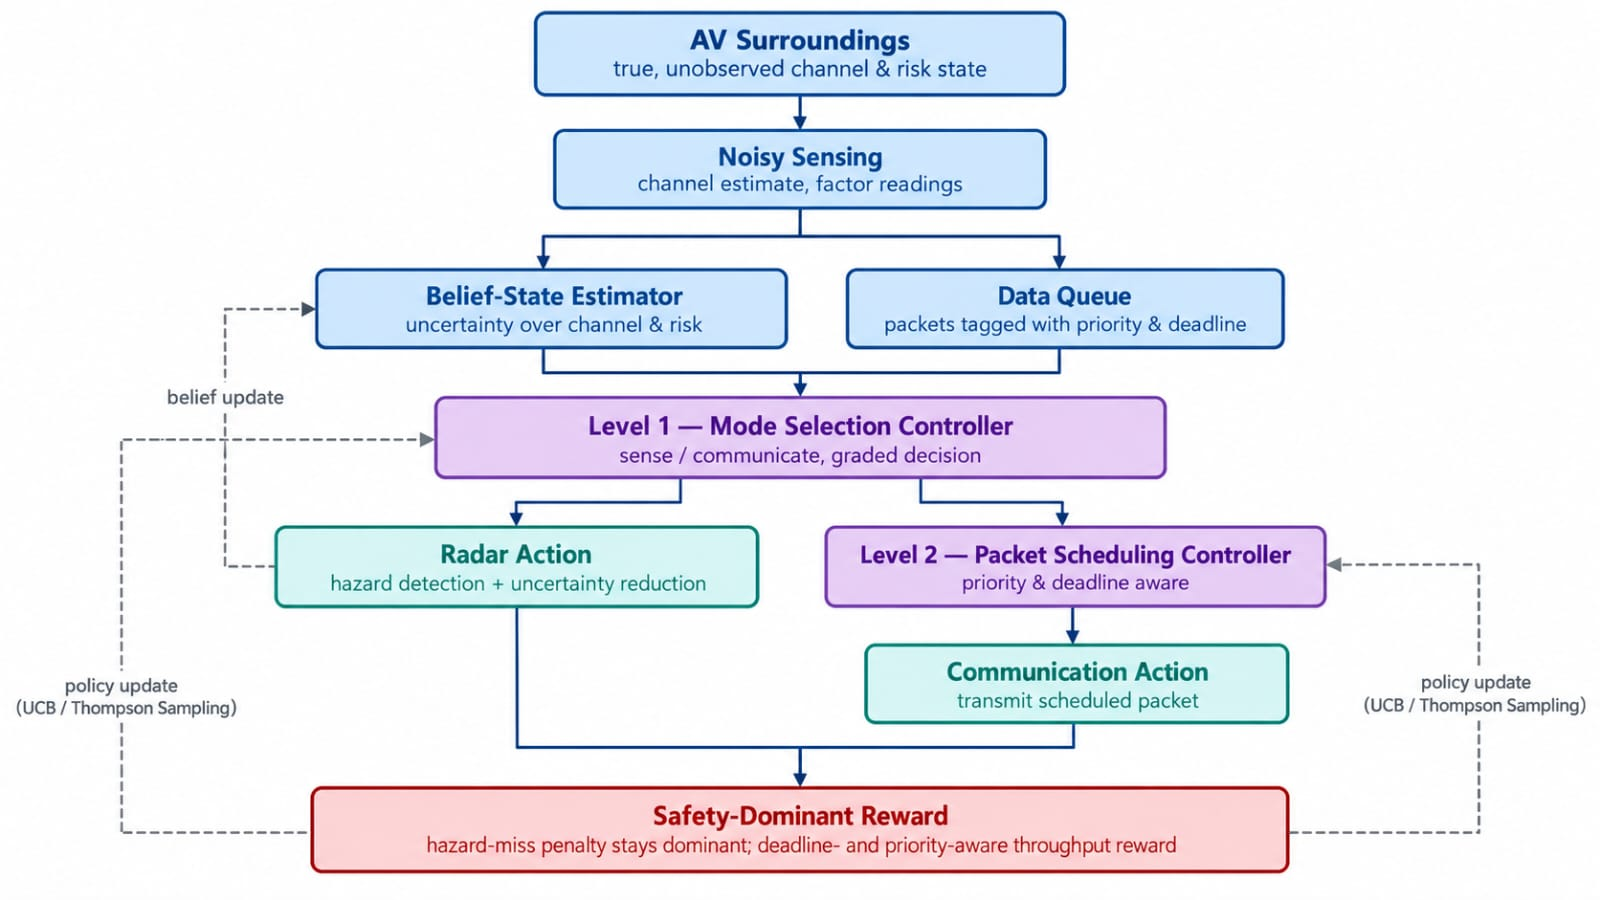
\includegraphics[height=5.5cm]{architecture/architecture.jpeg}
\end{frame}

% ============================================================================
% =====================  ARCHITECTURE EXPLAINED  =============================
% ============================================================================
\begin{frame}{Proposed Work: Research Methodology --- Architecture Explained}
  \footnotesize
  \begin{itemize}
    \setlength{\itemsep}{0.06cm}
    \item \textbf{AV Surroundings $\to$ Noisy Sensing}
      \begin{itemize}
        \small \item[--] True channel \& risk state is never observed directly, only sensed with noise
      \end{itemize}
    \item \textbf{Belief-State Estimator}
      \begin{itemize}
        \small \item[--] Maintains an uncertainty-aware estimate instead of assuming perfect knowledge
      \end{itemize}
    \item \textbf{Data Queue}
      \begin{itemize}
        \small \item[--] Packets are now tagged with priority and deadline, not just counted
      \end{itemize}
    \item \textbf{Level 1 --- Mode Selection Controller}
      \begin{itemize}
        \small \item[--] Decides sense vs.\ communicate as a graded decision, using belief + queue as context
      \end{itemize}
    \item \textbf{Radar Action}
      \begin{itemize}
        \small \item[--] Dual role: detects hazards \emph{and} feeds a belief update back to the estimator
      \end{itemize}
    \item \textbf{Level 2 --- Packet Scheduling Controller}
      \begin{itemize}
        \small \item[--] When communicating, picks which packet to send based on priority \& deadline
      \end{itemize}
    \item \textbf{Safety-Dominant Reward}
      \begin{itemize}
        \small \item[--] Hazard-miss penalty stays dominant; trains both controllers via UCB / Thompson Sampling
      \end{itemize}
  \end{itemize}
\end{frame}

% ============================================================================
% ==================  BASE PAPER: MDP FORMULATION  ============================
% ============================================================================
\begin{frame}{Base Paper: MDP Formulation (Sections II--III)}
  \footnotesize
  \textbf{The MDP tuple:} $\langle S, A, R, P \rangle$

  \begin{itemize}
    \setlength{\itemsep}{0.06cm}
    \item \textbf{State space $S$} (Eq.~2): $(d,c,r,w,v,m)$, $d\in\{0,\ldots,10\}$, others binary $\rightarrow$ \textbf{352 states}
    \item \textbf{Action space $A$}: $a=0$ (communicate) or $a=1$ (radar)
    \item \textbf{Environment model} (Eq.~1): $P(\oplus) = \sum_{i} \left[\tau_i p_0^i + (1-\tau_i)p_1^i\right]$, $i\in\{r,w,v,m\}$
    \item \textbf{Reward function} (Eq.~3): $+r_1$/$+r_2$ (comm, no event, good/bad channel); $-r_3$ (comm, event); $+r_4(b{+}1)$ (radar, event); $0$ (radar, no event)
    \item \textbf{Objective} (Eq.~4): $\displaystyle\max_\pi G(\pi) = \mathbb{E}\Big\{\sum_{t} \gamma^t r_{t+1}(\pi)\Big\}$
  \end{itemize}

  \vspace{0.25cm}
  \textbf{Scope of this review:} Implemented in full --- state space, action space, environment model, reward function, and objective --- everything through the end of Section III. Section IV (the DQN algorithm) is Phase 3.
\end{frame}

% ============================================================================
% ==================  PHASE 2 RESULTS  ========================================
% ============================================================================
\begin{frame}{Phase 2 Results: Environment Verification}
  \footnotesize
  \textbf{Sanity checks (MATLAB implementation):}
  \begin{itemize}
    \setlength{\itemsep}{0.04cm}
    \item State space size: \textbf{352} (matches Eq.~2 exactly)
    \item $P(\oplus)$ computed from Eq.~1: \textbf{0.1002}
  \end{itemize}

  \vspace{0.25cm}
  \textbf{Three fixed policies compared ($T=500$ steps, no learning yet):}
  \begin{center}
  \begin{tabular}{lrrrr}
    \toprule
    \textbf{Policy} & \textbf{Total Reward} & \textbf{Discounted $G$} & \textbf{Mean $d$} & \textbf{Events} \\
    \midrule
    Round-robin   & $-302.00$  & $-42.19$  & $1.58$ & $48/500$ \\
    Always-comm   & $-2044.00$ & $-546.83$ & $0.96$ & $58/500$ \\
    Always-radar  & $+595.00$  & $+105.75$ & $9.90$ & $49/500$ \\
    \bottomrule
  \end{tabular}
  \end{center}

  \vspace{0.2cm}
  \textbf{Inference:} Always-radar avoids the $-r_3$ penalty entirely but leaves the queue saturated (near-zero throughput). Always-comm drains the queue but repeatedly eats the $-50$ penalty. Round-robin sits between the two --- exactly the throughput/safety trade-off the reward function is designed to expose, and exactly what a learned policy (Phase 3) must resolve.
\end{frame}

% ============================================================================
% ===========================  PROJECT TIMELINE  =============================
% ============================================================================
\begin{frame}{Requisites Analysis and Project Plan}
  \scriptsize
  \renewcommand{\arraystretch}{1.15}
  \begin{tabular}{@{}p{3.1cm}p{9.6cm}@{}}
    \toprule
    \textbf{Phase} & \textbf{Focus} \\
    \midrule
    \textbf{Phase 1} \textit{(Completed)} & Part 1 implementation of the base paper: state space (Eq.~2), action space, environment model / unexpected-event probability (Eq.~1), reward function (Eq.~3), and discounted-return objective (Eq.~4) --- the full simulation environment, up to but not including the DQN algorithm (Section~IV). \\
    \textbf{Phase 2} & Complete the base paper by implementing the DQN algorithm (Section~IV) and reproducing the iRDRC baseline results (Section~V); then stress-test it across many scenarios --- varying channel/event probabilities, reward weights, and environmental conditions --- to empirically identify its drawbacks: the perfect-knowledge assumption breaking under estimation noise, the rigidity of the binary action, and the absence of QoS-aware scheduling. \\
    \textbf{Phase 3} & Halfway implementation of the proposed work: belief-state estimator, dual-role radar action, and the Level~1 Mode Selection Controller; evaluate the initial improvement over the base paper's DQN baseline from Phase~2. \\
    \textbf{Phase 4} & Complete the proposed architecture --- Level~2 Packet Scheduling Controller, deadline-/priority-aware reward, and full hierarchical training (UCB / Thompson Sampling); run the full comparative evaluation and ablation studies against the base paper and the literature reviewed; consolidate results, write the thesis, and prepare the final defense. \\
    \bottomrule
  \end{tabular}
\end{frame}

% ============================================================================
% ===========================  EXPECTED OUTCOMES  =============================
% ============================================================================
\begin{frame}{Expected Outcomes}
  \footnotesize
  \begin{itemize}
    \setlength{\itemsep}{0.05cm}
    \item A validated uncertainty-aware formulation --- a belief-state estimator producing a usable channel/risk estimate instead of assuming perfect knowledge, with radar confirmed to serve a \textbf{dual role}: hazard detection \emph{and} measurable uncertainty reduction.
    \item Demonstrated benefit of a \textbf{graded, multi-level} mode-selection space over iRDRC's strict binary action.
    \item A learned hierarchical policy (mode-selection + scheduling controllers) that \textbf{outperforms all three Phase 2 baselines} in discounted return $G(\pi)$ --- exceeding even always-radar's safety-only ceiling ($G = +105.75$) --- while keeping \textbf{safety dominant throughout} and maintaining meaningful throughput.
    \item Reduced miss-detection probability vs.\ the iRDRC baseline, without sacrificing throughput the way always-radar does; faster convergence than a flat DQN over the same (or richer) state space.
    \item A working deadline- and priority-aware packet scheduler, with measurably better on-time delivery for high-priority packets than iRDRC's undifferentiated throughput model.
    \item A direct, quantitative comparison against the base paper and the three recent extensions reviewed, positioning this work's contribution within the current literature.
  \end{itemize}
\end{frame}

% ============================================================================
% ===========================  REFERENCES  ====================================
% ============================================================================
\begin{frame}{References}
  \footnotesize
  \begin{enumerate}
    \setlength{\itemsep}{0.15cm}
    \item N. Q. Hieu, D. T. Hoang, N. C. Luong, and D. Niyato, ``iRDRC: An Intelligent Real-Time Dual-Functional Radar-Communication System for Automotive Vehicles,'' \textit{IEEE Wireless Communications Letters}, vol. 9, no. 12, pp. 2140--2143, Dec. 2020.
    \item J. Lee, Y. Cheng, D. Niyato, Y. L. Guan, and D. Gonz\'alez G., ``Intelligent Resource Allocation in Joint Radar-Communication With Graph Neural Networks,'' \textit{IEEE Transactions on Vehicular Technology}, vol. 71, no. 10, pp. 11120--11135, Oct. 2022.
    \item X. Li, M. Chen, Y. Hu, Z. Zhang, D. Liu, and S. Mao, ``Jointly Optimizing Terahertz Based Sensing and Communications in Vehicular Networks: A Dynamic Graph Neural Network Approach,'' \textit{IEEE}, 2024.
    \item C. Liu, M. Xia, J. Zhao, H. Li, and Y. Gong, ``Optimal Resource Allocation for Integrated Sensing and Communications in Internet of Vehicles: A Deep Reinforcement Learning Approach,'' \textit{IEEE Transactions on Vehicular Technology}, 2024.
  \end{enumerate}
\end{frame}

% ============================================================================
% THANK YOU
% ============================================================================
\begin{frame}[plain]
  \vspace{2cm}
  \begin{center}
    {\Huge\bfseries\color{iiitblue} Thank You}
    \vspace{1.5cm}

    {\Large\textit{Questions \& Discussion}}
  \end{center}
\end{frame}

\end{document}
